

\chapter{Week3}

\section{Monday}\index{Monday_lecture}
\subsection{Uniqueness of first ODE (Include non-linear)}
\paragraph{Question statement:}
Consider \[\left \{	\begin{gathered}
y^\prime=f(t,y)	\\
f(t_0)=y_0.
\end{gathered}\right.\] There exists a unique function $y$ that satisfies those equations near $(t_0,y_0)$\\
Before the proof begin, there is something need to be clarified. First $f$ and $f_y$ are continuous function on $\mathcal{R}:[t_0-a,t_0+a]\times[y_0-b,y_0+b]$ (a set of point that constitudes a rectangular area). Second $M=\sup_R|f(t,y)|$ $L=\sup_R|f_y(t,y)|$ ( $f_y$ means $\frac{\partial f}{\partial y}$).
\begin{figure}[H]
\centering
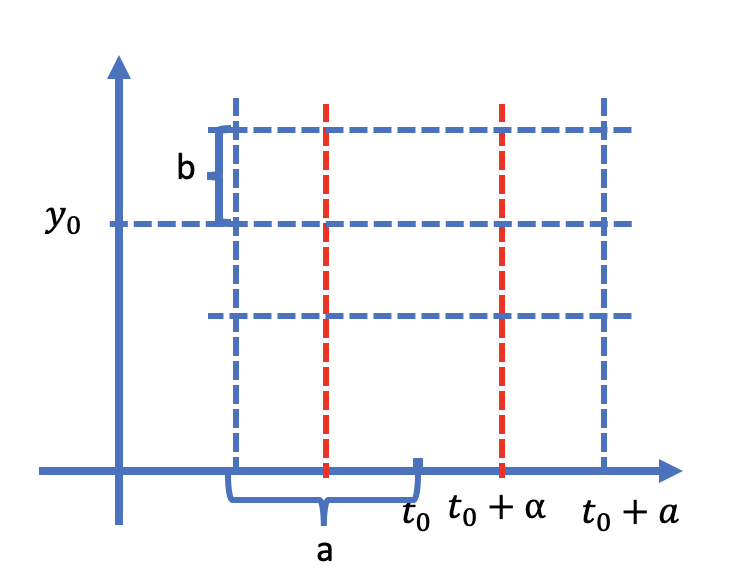
\includegraphics[width=8cm]{week3_mon}
\caption{Domain}
\end{figure}
\begin{proof}
Existence: $\exists \alpha>0$, s.t. ODE has a solution on $(t_0-\alpha,t_0+\alpha)$.
There are two methods mentioned during lecutre. The first is the one using contraction mapping. The other is \textbf{Picard iteration}:(set $t_0=0$)
Observe that:
\[y(t)-y(0)=\int_0^tf(s,y(s))\diff s 
\]
\[y(t)=y(0)+\int_0^tf(s,y(s))\diff s
\]
This equation has the same solution as the ODE. (Why is that? Think about it.) We are looking to this integral equation which are continuous.
Approximating solutions \[y_0(t)=y_0\quad\forall t\]
\[y_1(t)=y_0+\int_0^tf(s,y(s))\diff s
\]
\[\dots
\]
\[y_{n+1}(t)=y_0+\int_0^tf(s,y_n(s))\diff s
\]
\[\dots
\]
\[\{y_0,y_1,y_2,\dots,y_n,\dots\}
\]
If the sequence of those functions converges uniformly, say it converges to $g$. Then we can find out that g is the function we are looking for. ($\lim_{n+1\rightarrow\infty}y_{n+1}(t)=y_0+\lim_{n\rightarrow\infty}\int_0^tf(s,y_n(s))\diff s$). W.T.S. uniform convergnece:\\
\[y_n(t)=y_0(t)+(y_1(t)-y_0(t))+\dots+(y_n(t)-y_{n-1}(t))
\]Without loss of generality, consider $t>0$
\[|y_1(t)-y_0(t)|\leq\int_0^t|f(s,y_0(s))|\diff t\leq M\int_0^t\diff s=Mt\quad\dots (1)
\]
\[\begin{aligned}|y_2-y_1(t)|&\leq\int_0^t|f(s,y_1(s)-f(s,y_0(s))|\diff s\\
&=\int_0^t|f_y(s,\xi(s))||y_1(s)-y_0(s)|\diff s \qquad\text{mean value theorem}\\
&\leq LM\int_0^ts\diff s=\frac{LMt^2}{2}\qquad\text{with (1)}
\end{aligned}
\]
\[
\begin{aligned}|y_3(t)-y_2(t)|&\leq\int_0^t|f(s,y_2(s))-f(s,y_1(s))|\diff s\\
&=\int_0^t|f_y(s,\xi_1(s))||y_2(s)-y_1(s)|\diff s\\
&\leq\frac{L^2M}{2}\int_0^ts^2\diff s=\frac{L^2Mt^3}{s\cdotp2\cdotp1}
\end{aligned}
\]
The same computation implies $|y_n(t)-y_{n-1}(t)|\leq\frac{L^{n-1}M}{n!}t^n$.\\
Claim $\{y_0, y_1, y_2, \dots, y_n, \dots\}$ is a Cauchy sequence i.e. for $|t|\leq\alpha$ $n>m$ 
\[\begin{aligned}
|y_n(t)-y_m(t)|
&\leq|y_n(t)-y_{n-1}(t)|+|y_{n-1}(t)-y_{n-2}(t)|+\cdots+|y_{m+1}(t)-y_{m}(t)|\\
&\leq\frac{L^{n-1}M}{n!}t^n+\frac{L^{n-2}M}{(n-1)!}t^{n-1}+\cdots+\frac{L^{m}M}{(m+1)!}t^{m+1}\\
&\leq\frac{M}{L}[e^{Lt}-(1+Lt+\cdots+\frac{(Lt)^m}{m!})]\qquad\text{Taylor expansion}\\
&\leq\frac{M}{L}[e^{L\alpha}-(1+L\alpha+\cdots+\frac{(L\alpha)^m}{m!})]\rightarrow 0 \text{ as } m\rightarrow\infty
\end{aligned}
\]
Before moving to prove the uniqueness of the solution, let's have a look at why the solution can only be gotten within a small neighbourhood ($t<|\alpha|$). The leak appear when we use mean value theorem. $\xi_n(s)$, the partial $y$ direvative of $f$, which is between $y_{n+1}(s)$  and $y_n(s)$ need to be inside the domain. This is the same as every $y_n(s)$ needs to be inside domain.( Shown by induction)\\
\[|y_1(t)-y_0(t)|\leq\int_0^t|f(s,y_0(s))|\diff s\leq M\int_0^t\diff s=Mt\leq M\alpha\leq b
\]
\[|y_{n+1}-y_0|\leq\int_0^t|f(s,y_n(s))|\diff s\leq M\int_0^t\diff s=Mt\leq M\alpha<b
\]
\[y_{n+1}=y_0+\int_0^tf(s,y_n(s))\diff s
\]
Therefore, every $y_n$ lies in $|t_0|<\alpha$.\\
\textbf{Uniqueness}\\
Suppose the ODE has two sols $y_1$ and $y_2$
\[y_1(t)=y_0+\int_0^tf(s,y_1(s))\diff s
\]
\[y_2(t)=y_0+\int_0^tf(s,y_2(s))\diff s
\]
\[\begin{aligned}|(y_1-y_2)(t)|&\leq\int_0^t|f(s,y_1(s))-f(s,y_2(s))|,(t>0)\\
&\leq\int_0^t|f_y(s,\xi(s))||y_1(s)-y_2(s)|\diff s
\end{aligned}
\]
\[|(y_1-y_2)(t)|\leq\int_0^t|y_1(s)-y_2(s)|\diff s\qquad |t|\leq\alpha\qquad\dots(2)
\]
Set $z(t)=\int_0^t|y_1(t)-y_2(t)|\diff s$ $\Rightarrow$ $z^\prime(t)=|y_1(t)-y_2(t)|\leq Lz(t)$ by (2)
\[z^\prime(t)-Lz(t)\leq0
\]
\[|e^{-Lt}z(t)|^\prime\leq0
\]
\[e^{-Lt}z(t)\leq0
\]
\[z(t)\leq0\quad\Rightarrow|y_1(s)-y_2(s)|=0
\]


\end{proof}
 \begin{example}
 \[y^\prime=\frac{3}{2}y^{\frac{1}{3}}
 \]
 $y\equiv0$ and  $y=t^{\frac{3}{2}}$ are solutions of above. Why this is the case? We just proved uniqueness of ODE.\\ The reason is that it doesn't fit the assumption that $f_y$ is continuous.
 \end{example}
 
 
 
 
 